\section{Basics}

\begin{frame}[fragile]
  \frametitle{C++ Compiler}
  \begin{center}
  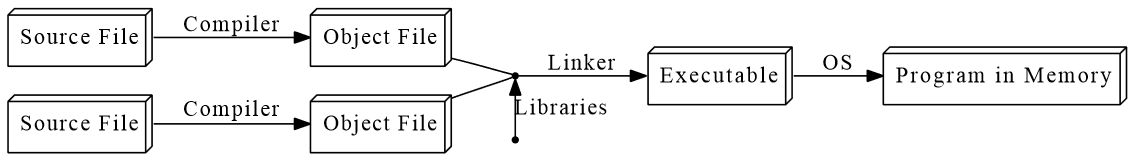
\includegraphics[scale=0.35]{img/compiler.png}
  \end{center}
  \vspace{1mm}
  Commands (GNU C++ Compiler):
  \begin{itemize}
  \item \verb|g++ source.cpp|\\
  {\tiny Compiles and links the source file. An executable file \verb|a.exe| (Windows) or \verb|a.out|
  (Linux) will be created.}
  \item \verb|g++ -c source.cpp|\\
  {\tiny Compiles the source file. An object file \verb|source.o| will be created.}
  \item \verb|g++ -o file.exe source.cpp|\\
  {\tiny Compiles and links the source file. An executable file \verb|file.exe| will be created.}
  \item \verb|g++ -std=c++14 source.cpp|\\
  {\tiny Compiles and links the source file by using the C++ 2014 standard.}
  \end{itemize}
\end{frame}

\begin{frame}[fragile]
  \frametitle{Hello World}
  A Hello World program is a computer program that outputs \verb|"Hello, World!"|. Because this is
  typically the simplest program in most programming languages.
  {\tiny
  \lstinputlisting{code/hello.cpp}
  }
\end{frame}

\begin{frame}[fragile]
  \frametitle{Variables, Datatypes}
  Declaration:
  {\small
\begin{lstlisting}
int n; // one variable with the name n
int a, b; // two variables

// variable with c-like initialization
float x = 5;

// variable with constructor initialization
float y(0);

// variable with uniform initialization (C++ 2011)
float z{0};
\end{lstlisting}
  }
  {\bf A variable will not be initialized!}
\end{frame}

\begin{frame}[fragile]
  \frametitle{Variables, Datatypes}
  Declaration:
  {\small
\begin{lstlisting}
double myNumber;

// var will be an integer, same as a (C++ 2011)
int a = 10;
auto var = a;

// constant. variable which cannot be changed
const int v = 10;
\end{lstlisting}
}
  {\bf A variable will not be initialized!}
\end{frame}

\begin{frame}[fragile]
  \frametitle{Variables, Datatypes}
  {\scriptsize
  \begin{tabular}{|l|l|l|}
  \hline
  \emph{Datatype} & \emph{Number of Bytes} & \emph{Values} \\
  \hline
  \verb|char| & 1 & single character\\
  \verb|int| & 4 & numerical integer type\\
  \verb|long int| & 4 & numerical integer type\\
  \verb|long long int| & 8 & numerical integer type\\
  \verb|short int| & 2 & numerical integer type\\
  \verb|float| & 4 & floating point type\\
  \verb|double| & 8 & floating point type\\
  \verb|bool| & 1 & boolean type \verb|true| or \verb|false|\\
  \hline
  \end{tabular}
  }
  \par
  The number of used bytes is dependent on the compiler and the operating system!
\end{frame}

\begin{frame}[fragile]
  \frametitle{Variables, Datatypes}
  {\scriptsize
  \begin{tabular}{|l|l|l|}
  \hline
  \emph{Datatype} & \emph{Number of Bytes} & \emph{Values} \\
  \hline
  \verb|unsigned char| & 1 & single character\\
  \verb|unsigned int| & 4 & numerical integer type\\
  \verb|unsigend long int| & 4 & numerical integer type\\
  \verb|unsigend long long int| & 8 & numerical integer type\\
  \verb|unsigend short int| & 2 & numerical integer type\\
  \hline
  \end{tabular}
  }
  \par
  The number of used bytes is dependent on the compiler and the operating system!
\end{frame}

\begin{frame}[fragile]
  \frametitle{Variables, Datatypes - Exercise}
  \begin{exercise}
  Write a program which prints out the number of used bytes for each datatype.
  \end{exercise}
\end{frame}

\begin{frame}[fragile]
  \frametitle{Variables, Datatypes - Exercise}
  \begin{exercise}
  A bool variable needs 1 Byte in memory. 1 Byte are 8 Bits. Why does a bool
  variable needs 8 Bits? As there are only two states (\verb|true| and \verb|false|) one Bit
  should be sufficient.
  \end{exercise}
\end{frame}

\begin{frame}[fragile]
	\frametitle{C++ Operators - Assignment}
	The assignment operator \verb|=| assigns a value to a variable.

	\vspace{3mm}

\begin{lstlisting}
a = 5;
\end{lstlisting}
\end{frame}

\begin{frame}[fragile]
	\frametitle{C++ Operators - Arithmetic}
	\begin{itemize}
	\item \verb|+  | Addition
	\item \verb|-  | Subtraction
	\item \verb|*  | Multiplication
	\item \verb|/  | Division
	\item \verb|%  | Modulo
	\item \verb|+= | \verb|i+=7| identical with \verb|i=i+7|
	\item \verb|-= | \verb|i-=7| identical with \verb|i=i-7|
	\item \verb|*= | \verb|i*=7| identical with \verb|i=i*7|
	\item \verb|/= | \verb|i/=7| identical with \verb|i=i/7|
	\item \verb|%= | \verb|i%=7| identical with \verb|i=i%7|
	\end{itemize}
\end{frame}

\begin{frame}[fragile]
	\frametitle{C++ Operators - Increment/Decrement}
	The increase operator \verb|++| and the decrease operator \verb|--| increase or
reduce by one the value stored in a variable.

	\vspace{5mm}

	\verb|i++  | is identical with \verb|i = i + 1|\\
	\verb|i--  | is identical with \verb|i = i - 1|
\end{frame}

\begin{frame}[fragile]
	\frametitle{C++ Operators - Relational}
	Two expressions can be compared using relational and equality operators.
	\begin{itemize}
	\item \verb|== | Equal to
	\item \verb|!= | Not equal to
	\item \verb|>  | Greater than
	\item \verb|<  | Less than
	\item \verb|>= | Greater than or equal to
	\item \verb|<= | Less than or equal to
	\end{itemize}
\end{frame}

\begin{frame}[fragile]
	\frametitle{C++ Operators - Logical}
	The following logical operators are available:

	\begin{itemize}
	\item \verb|!           Not|
	\item \verb|&&          And|
	\item \begin{verbatim}||          Or\end{verbatim}
	\end{itemize}
\end{frame}

\begin{frame}[fragile]
  \frametitle{C++ Operators - Exercise}
  \begin{exercise}
  What is the content of variable \verb|r|?
\begin{lstlisting}
int a = 5, b = 6, c = 7;
bool d = true, e = false;
bool r = (a == b || d) && (c >= 7 && !e);
\end{lstlisting}
  \end{exercise}
\end{frame}

\begin{frame}[fragile]
  \frametitle{Input,Output}
  Streams available in the standard library:
  \begin{itemize}
  \item cin (standard input stream)
  \item cout (standard output stream)
  \item cerr (standard error stream)
  \item clog (standard logging stream)
  \end{itemize}
\end{frame}

\begin{frame}[fragile]
  \frametitle{Input,Output}
  In most program environments, the standard output by default is the screen,
  and the C++ stream object defined to access it is cout.
  {\scriptsize
\begin{lstlisting}
cout << "some text..."; // prints some text... on the screen
cout << 23; // prints the number 23 on the screen
cout << x; // prints the value of x on the screen
cout << "x = " << x << endl; // multiple insertions
\end{lstlisting}
  }
\end{frame}

\begin{frame}[fragile]
  \frametitle{Input,Output}
  In most program environments, the standard input by default is the keyboard,
  and the C++ stream object defined to access it is cin.
\begin{lstlisting}
int number;
cin >> number;
\end{lstlisting}
\end{frame}

\begin{frame}[fragile]
  \frametitle{Input,Output - Exercise}
  \begin{exercise}
  Write a program which reads the height of a satellite and prints out
  the time used for one rotation of the earth.\\
  The formulae to calculate the time is
  \begin{displaymath}
T[sec] = \frac{2 \cdot \pi}{R_{E}} \cdot \sqrt{\frac{(R_{E}+h)^{3}}{g}}
\end{displaymath}

$g$ is the acceleration of gravity: $g = 9.80665 m/s^{2}$\\
$R_{E}$ radius of the earth: $R_{E} = 6371 km$\\
$\pi = 3.14159$\\
  \end{exercise}
\end{frame}

\begin{frame}[fragile]
  \frametitle{Selection}
  The if keyword is used to execute a statement or block, if, and only if, a condition is fulfilled. Its syntax is:
\begin{lstlisting}
if (condition) {
  // some code
}
\end{lstlisting}
Example:
\begin{lstlisting}
if (n == 100) {
  // some code
}
\end{lstlisting}
\end{frame}

\begin{frame}[fragile]
  \frametitle{Selection}
  {\scriptsize
  Selection statements with if can also specify what happens when the condition is not fulfilled,
  by using the else keyword to introduce an alternative statement. Its syntax is:
\begin{lstlisting}
if (condition) {
  // some code
} else {
  // some code
}
\end{lstlisting}
Several if + else structures can be concatenated with the intention of checking a range of values. For example:
\begin{lstlisting}
if (condition) {
  // some code
} else if (other_condition) {
  // some code
} else {
  // some code
}
\end{lstlisting}
}
\end{frame}

\begin{frame}[fragile]
  \frametitle{Switch}
  {\scriptsize
  \verb|switch| checks for a value among a number of possible constant expressions.
  It is something similar to concatenating if-else statements, but limited to constant expressions. 
  \begin{lstlisting}
switch (expression) {
  case constant1:
    some code 1;
    break;
  case constant2:
    some code 2;
    break;
  default:
    some code;
}
  \end{lstlisting}
  \verb|switch| evaluates the expression and checks if it is equivalent to
  \verb|constant1|. if it is, it executes \verb|some code 1| until it finds
  the break statement. When it finds this break statement, the program jumps
  to the end of the entire switch statement. If no constant will match the
  expression, the default case (if available) will be executed.
  }
\end{frame}

\begin{frame}[fragile]
  \frametitle{Switch}
  {\scriptsize
  \begin{lstlisting}
switch (x) {
  case 1:
  case 2:
    cout << "x is 1 or 2";
    break;
  case 3:
    cout << "x is 3";
    break;
  default:
    cout << "x is not 1, 2 nor 3";
  }
}
  \end{lstlisting}
  }
\end{frame}

\begin{frame}[fragile]
  \frametitle{Selection - Exercise}
  \begin{exercise}
  Write a program which defines if a year is a leap year.\\
  A year is a leap year
  \begin{itemize}
  \item if the year is a century, it must be divideable by 400
  \item else it must be divideable by 4
  \end{itemize}
  \end{exercise}
\end{frame}

\begin{frame}[fragile]
  \frametitle{Selection - Exercise}
  \begin{exercise}
  Write a 5 function simple calculator. The program reads two values (a, b) and
  an operator (+, -, *, /, p) from the commandline and calculates the output.\\
  The operators are defined as follows:
  \begin{itemize}
  \item $+: a+b$
  \item $-: a-b$
  \item $*: a\cdot b$
  \item $/: a \div b$
  \item $p: a^b$
  \end{itemize}
  \end{exercise}
\end{frame}


\begin{frame}[fragile]
  \frametitle{Iteration}
  Loops repeat a statement a certain number of times, or while a condition is fulfilled.
  They are introduced by the keywords
  \begin{itemize}
  \item while
  \item do-while
  \item for
  \end{itemize}
\end{frame}

\begin{frame}[fragile]
  \frametitle{Iteration}
  The simplest kind of loop is the while-loop. Its syntax is:
\begin{lstlisting}
while (condition) {
// some code
}
\end{lstlisting}
\end{frame}

\begin{frame}[fragile]
\frametitle{Iteration}
Calculate the following series until one element is $<0.0002$.
\begin{displaymath}
sum = \frac{1}{1} + \frac{1}{2} + \frac{1}{3} + \frac{1}{4} + ...
\end{displaymath}
{\tiny
\begin{lstlisting}
int main(int argc, char **argv) {
  double sum = 0;
  int dividend = 1;

  while (1.0/dividend >= 0.0002) {
    sum = sum + (1.0/dividend);
    dividend = dividend + 1;
  }
  cout << sum << endl;
  return 0;
}
\end{lstlisting}
}
\end{frame}

\begin{frame}[fragile]
  \frametitle{Iteration}
  A very similar loop is the do-while loop, whose syntax is:
\begin{lstlisting}
do {
  // some code
} while (condition);
\end{lstlisting}
\end{frame}

\begin{frame}[fragile]
  \frametitle{Iteration - Exercise}
  \begin{exercise}
  What is the difference between a while loop and a do-while loop?
  \end{exercise}
\end{frame}

\begin{frame}[fragile]
  \frametitle{Iteration}
  The for loop is designed to iterate a number of times. Its syntax is:
\begin{lstlisting}
for (initialization; condition; increase) {
  // some code
}
\end{lstlisting}
\end{frame}

\begin{frame}[fragile]
\frametitle{Iteration}
Calculate the first 100 members of the following series:
\begin{displaymath}
sum = \frac{1}{1} + \frac{1}{2} + \frac{1}{3} + \frac{1}{4} + ...
\end{displaymath}
\begin{lstlisting}
int main(int argc, char **argv) {
  double sum = 0;
  for (int i=0; i<100; i++) {
    sum = sum + (1.0/(i+1));
  }
  cout << sum << endl;
  return 0;
}
\end{lstlisting}
\end{frame}

\begin{frame}[fragile]
\frametitle{Iteration}
The for-loop has another syntax, which is used exclusively with ranges:
\begin{lstlisting}
for (declaration : range) {
  // some code
}
\end{lstlisting}
\end{frame}

\begin{frame}[fragile]
\frametitle{Iteration}
Loop through all characters of a string:
\begin{lstlisting}
int main(int argc, char **argv) {
  string str = "Hello World";
  for (char ch : str) {
    // some code
  }
  return 0;
}
\end{lstlisting}
\end{frame}

\begin{frame}[fragile]
\frametitle{Iteration - Exercise}
\begin{exercise}
Write a program which reads 10 numbers from the command line. At the end the program
will print the smallest of these 10 numbers.\\
\end{exercise}
\end{frame}

\begin{frame}[fragile]
\frametitle{Iteration - Exercise}
\begin{exercise}
Write a program which prints random numbers:\\
\begin{itemize}
\item 10 random numbers (integer)
\item 10 random numbers between 0 and 100 (integer)
\item 10 random numbers between 0 and 1 (float)
\end{itemize}
{\tiny
\begin{lstlisting}
#include <cstdlib>
using namespace std;

// creates a random number between 0 and RAND_MAX
int number = rand();

// prints RAND_MAX
cout << RAND_MAX << endl;
\end{lstlisting}
}
How big is \verb|RAND_MAX|?
\end{exercise}
\end{frame}


\begin{frame}[fragile]
\frametitle{Iteration - Exercise}
\begin{exercise}
Write a program which simulates the galton board for 100 balls.\\
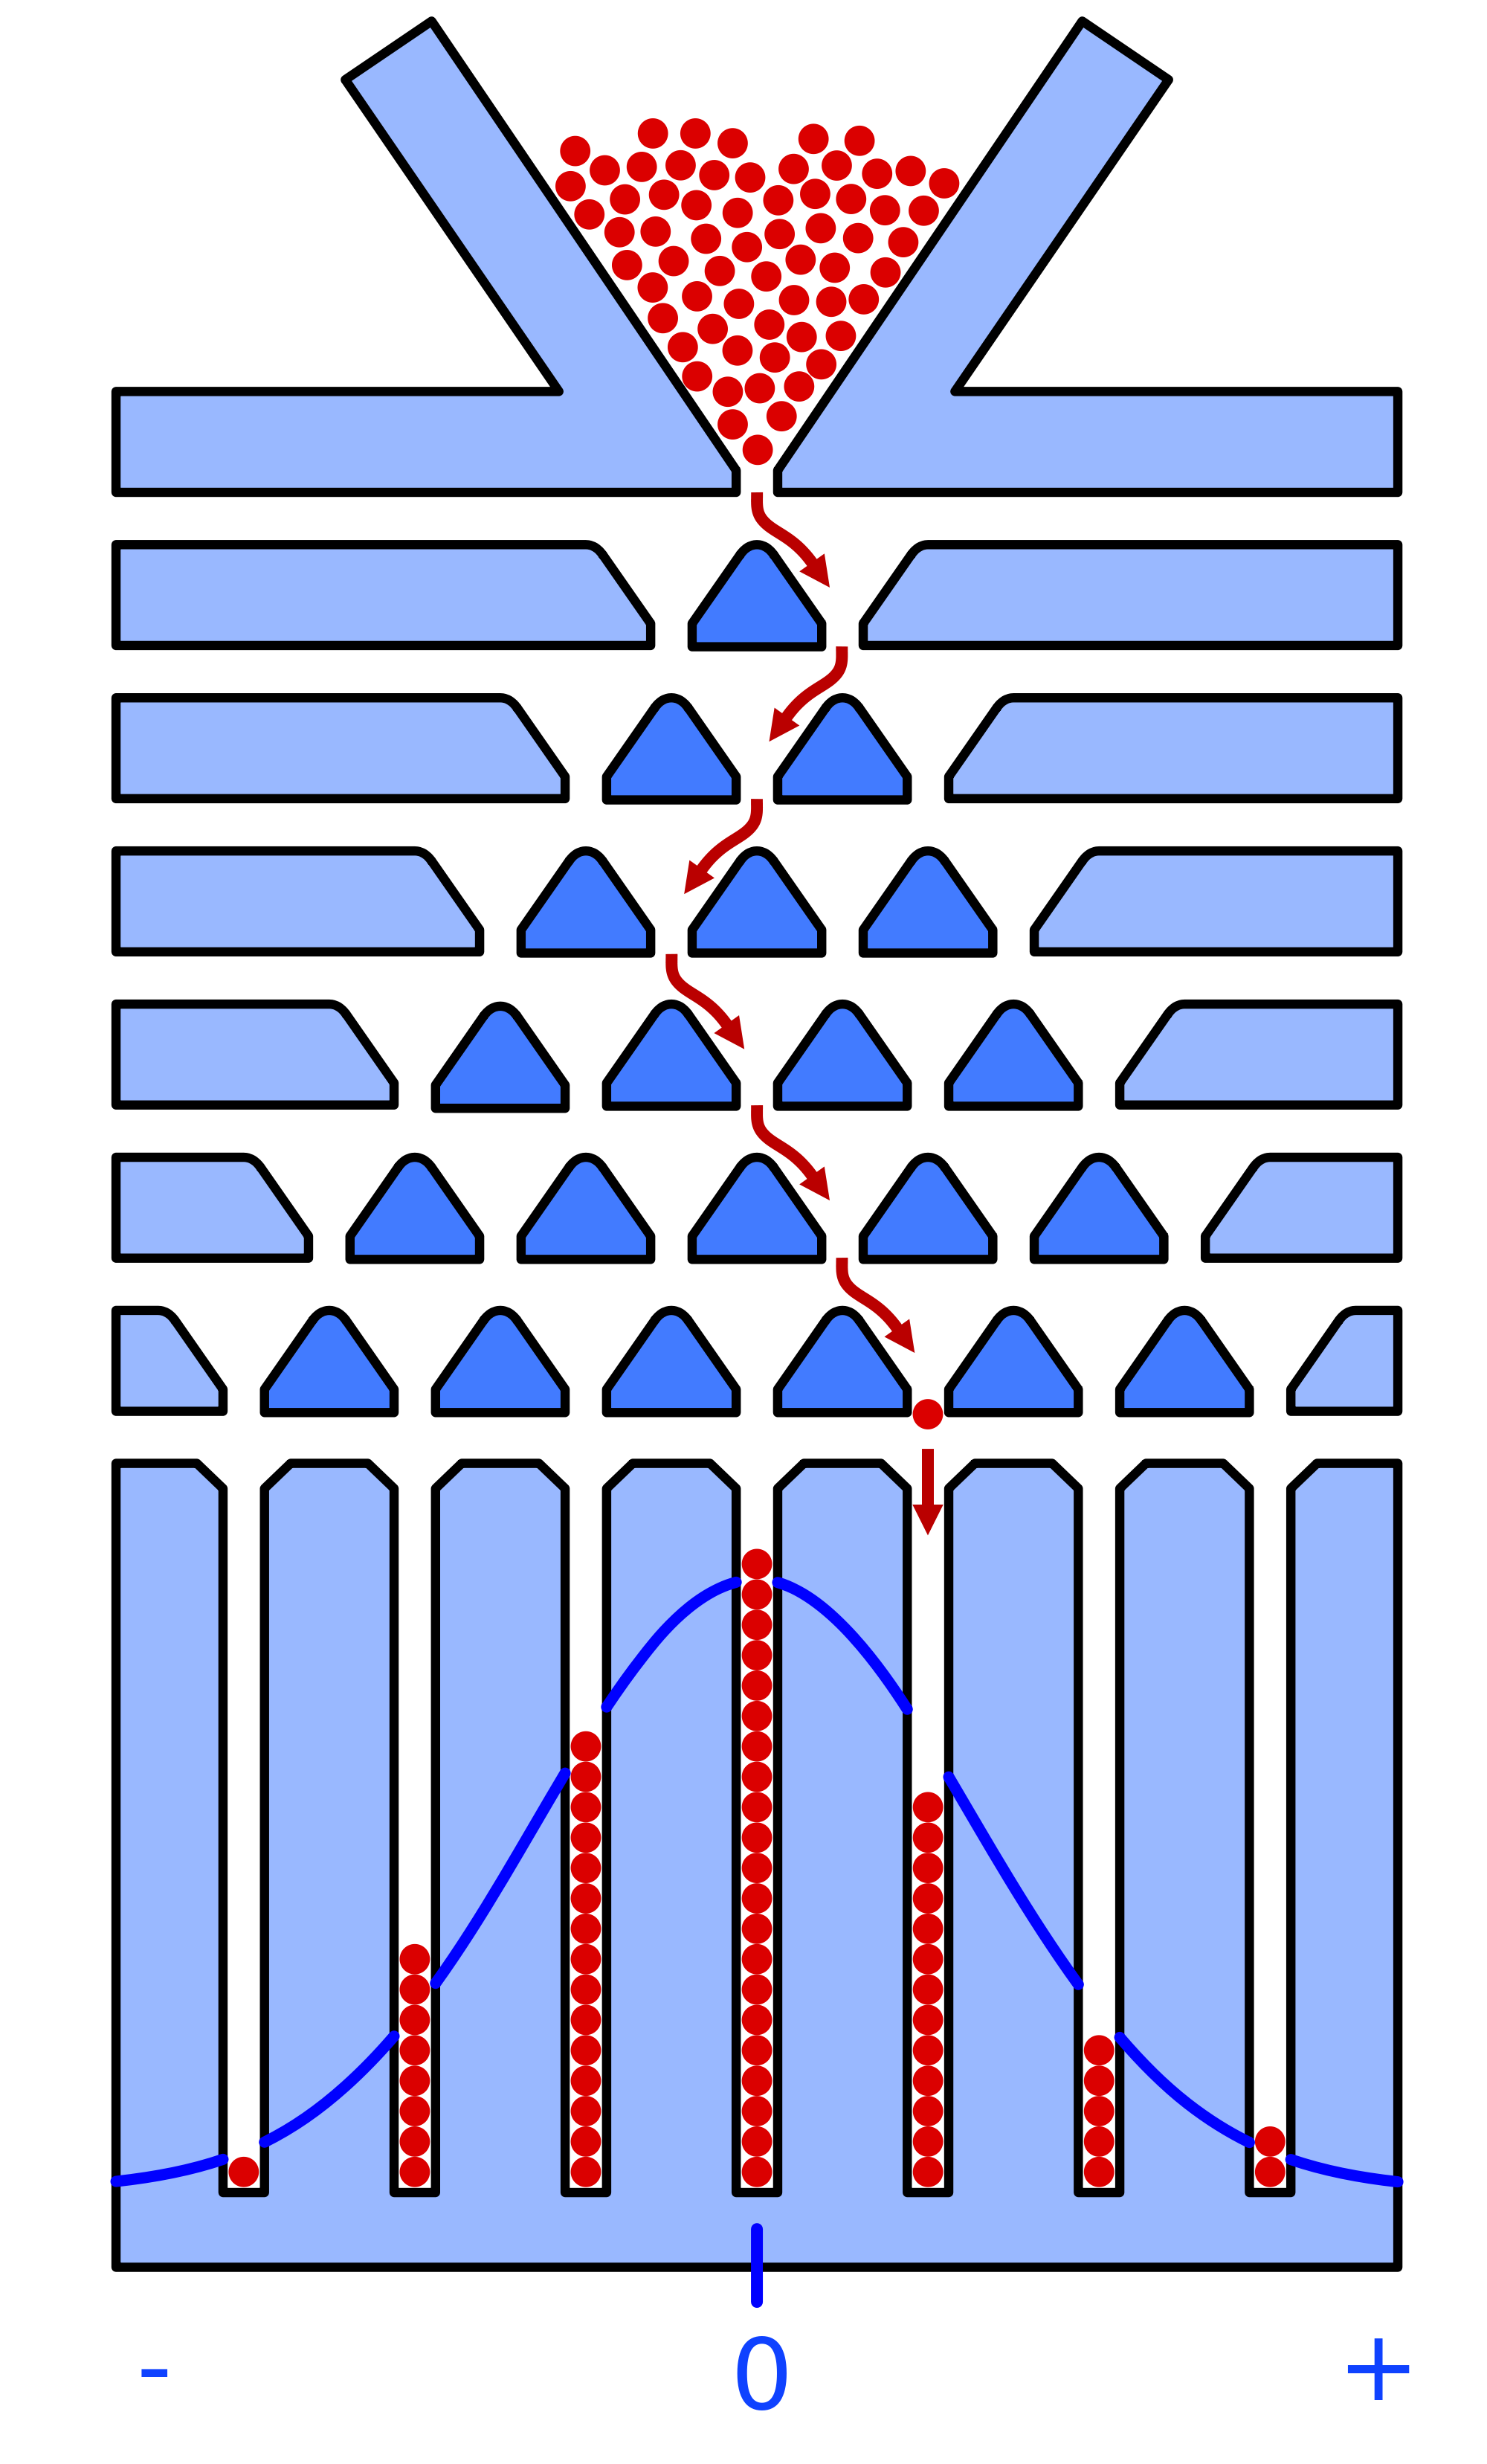
\includegraphics[scale=0.04]{img/galton.png}
\end{exercise}
\end{frame}

\begin{frame}[fragile]
\frametitle{Iteration - Exercise}
\begin{exercise}
Write a program which simulates the probability of having a blackjack (Ace and 10).
The game contains 6 sets of cards. Each set has 52 cards.\\

\includegraphics[scale=0.5]{img/blackjack.jpg}
\end{exercise}
\end{frame}


\begin{frame}[fragile]
  \frametitle{Jump}
  Jump statements allow altering the flow of a program by performing jumps to specific locations.
  \begin{itemize}
  \item {\bf break}\\
  break leaves a loop, even if the condition for its end is not fulfilled.
  It can be used to end an infinite loop, or to force it to end before its natural end.
  \item {\bf continue}\\
  The continue statement causes the program to skip the rest of the loop in the current iteration, as if the end of the statement block had been reached,
  causing it to jump to the start of the following iteration.
  \end{itemize}
\end{frame}

\begin{frame}[fragile]
\frametitle{Arrays}
An array is a series of elements of the same type placed in contiguous memory locations that can
be individually referenced by adding an index to a unique identifier.
\begin{lstlisting}
int a[5]; // creates 5 variables of type int
a[0] = 0;
a[1] = 1;
...
a[4] = 4;
\end{lstlisting}
ATTENTION: read or write access to an element which is not in the range of the array
end up in serious problems!
\end{frame}

\begin{frame}[fragile]
\frametitle{Arrays - Initialization}
By default, arrays are left uninitialized. This means that none of its elements are set to any particular value.
\begin{lstlisting}
int a[5] = {0, 1, 2, 3, 4};
\end{lstlisting}

Values which are not provided in the initialization list will be filled up with zeros.
\begin{lstlisting}
int b[5] = {0, 1};
\end{lstlisting}

Empty initialization list. All elements will have the value 0.
\begin{lstlisting}
int c[5] = {};
\end{lstlisting}

Array without a given size
\begin{lstlisting}
int d[] = {0, 1, 2};
\end{lstlisting}

\end{frame}

\begin{frame}[fragile]
\frametitle{Arrays - Example}
\lstinputlisting{code/array/main.cpp}
\end{frame}

\begin{frame}[fragile]
\frametitle{Arrays - Multidimension}
Arrays in C++ could have several dimensions.
\lstinputlisting{code/array/multiarray.cpp}
\end{frame}

\begin{frame}[fragile]
\frametitle{Strings}
A string is traditionally a sequence of characters. C++ provides two types for string representations:
\begin{itemize}
\item C-Style character array
\item String class from C++ Standard
\end{itemize}
\end{frame}

\begin{frame}[fragile]
\frametitle{Strings - Character Array}
The C-style character string (\verb|#include<cstring>|) originated within the C language and continues to be supported within C++.
This string is actually a one-dimensional array of characters which is terminated by a null
character \verb|\0|.
\begin{lstlisting}
char s1[6] = {'H', 'e', 'l', 'l', 'o', '\0'};
char s2[] = "Hello";
\end{lstlisting}
Several operations are available, e.g. \verb|strcpy|, \verb|strcat|, \verb|strlen|, ...
\end{frame}

\begin{frame}[fragile]
\frametitle{Strings - String class}
The standard C++ library (\verb|#include<string>|) provides a string class that supports much more operations
as the old C-String.
\begin{lstlisting}
string s1 = "Hello";
string s2 = "World";
cout << s1.size() << endl;
\end{lstlisting}
A more detailed introduction to strings will be part in the STL chapter.
\end{frame}

\begin{frame}[fragile]
\frametitle{Strings - Exercise}
\begin{exercise}
Write a program which takes a string as input. The string contains a set of pairs. Each
pair contains a number and a character: \verb|2n3m5x| (3 pairs: 2n, 3m and 5x).\\
The program should now encode this string by writing all character the given amount
of times.\\
\verb|2n3m5x| will be \verb|nnmmmxxxxx|.
\end{exercise}
\end{frame}

\begin{frame}[fragile]
\frametitle{Pointers}
When a variable is declared, the memory needed to store its value to a specific location in memory.
The exact position is defined by the operating system. However, it may be useful for a program to be
able to obtain the memory address of a variable during runtime in order to access data cells that
are at a certain position relative to it.\\
\vspace{3mm}
The address operator \verb|&| is used to find out the address in memory of a variable.

{\tiny
\begin{lstlisting}
int n = 5; // integer variable
int *p; // pointer variable. Stores the address of an integer variable
p = &n; // Stores the address of n into p
cout << p << endl; // print the address of n
\end{lstlisting}
}
\end{frame}

\begin{frame}[fragile]
\frametitle{Pointers}
The dereference operator \verb|*| is used to access a variable by using its address.

{\tiny
\begin{lstlisting}
int n = 5; // integer variable
int *p; // pointer variable. Stores the address of an integer variable
p = &n; // Stores the address of n into p
n = 20; // Stores 20 in n by using the variable name
*p = 25; // Stores 25 in n by using the variable address
\end{lstlisting}
}
\end{frame}

\begin{frame}[fragile]
\frametitle{Pointers}
Defining pointer variables:
{\tiny
\begin{lstlisting}
int *p; // defines a pointer to store the address of a int variable
int *n, m; // n is a pointer, m is NOT a pointer
float *fp; // defines a pointer to store the address of a float variable
\end{lstlisting}
}
\end{frame}

\begin{frame}[fragile]
\frametitle{Pointers}
In principle, pointers are meant to point to valid addresses,
such as the address of a variable or the address of an element in an array.
But pointers can actually point to any address,
including addresses that do not refer to any valid element. 
{\tiny
\begin{lstlisting}
int *p; // undefined pointer
*p = 5;
\end{lstlisting}
}
Accessing such a pointer causes undefined behavior,
ranging from an error during runtime to accessing some random value.
\end{frame}

\begin{frame}[fragile]
\frametitle{Pointers}
But, sometimes, a pointer really needs to explicitly point to nowhere, and not just an invalid address.
For such cases, there exists a special value that any pointer type can take:
the null pointer value.
{\tiny
\begin{lstlisting}
int *p;
p = 0;
p = nullptr;
p = NULL;
\end{lstlisting}
}
Accessing such a pointer causes undefined behavior,
ranging from an error during runtime to accessing some random value.
\end{frame}

\begin{frame}[fragile]
\frametitle{Dynamic Memory}
In the programs seen in previous slides, all memory needs were determined
before program execution by defining the variables needed.
But there may be cases where the memory needs of a program can only be determined during runtime.

\begin{lstlisting}
int *p = null; // pointer variable
p = new int;
// creates a new integer variable,
// p will now point to this variable
\end{lstlisting}

\begin{lstlisting}
int *p = null; // pointer variable
p = new int[5];
// creates a new integer array,
// p will now point to p[0]
\end{lstlisting}

\end{frame}

\begin{frame}[fragile]
\frametitle{Dynamic Memory}
Dynamic memory is in most cases only needed for a specific period of time within
the program. The allocated memory needs then to be released.

\begin{lstlisting}
int *p = null; // pointer variable
p = new int;
// some code
delete p;
// the memory to which p points will be
// released. The pointer p will still exist.
\end{lstlisting}
\end{frame}

\begin{lstlisting}
int *p = null; // pointer variable
p = new int[5];
// some code
delete [] p;
\end{lstlisting}

\begin{frame}[fragile]
\frametitle{Dynamic Memory}
Memory Leaks:

\begin{lstlisting}
int *p = null; // pointer variable
p = new int;
// some code
p = new int;
\end{lstlisting}
In the above code, the first allocated memory will be lost
after the second allocation.\\
This means that the variable is still in there, but unknown where
in the memory. This is called \bf{Memory Leak}.

\end{frame}

\begin{frame}[fragile]
\frametitle{References}
A reference variable is an alias, that is, another name for an already existing
variable.
\begin{lstlisting}
int i = 17;
int &r = i;
\end{lstlisting}
\end{frame}

\begin{frame}[fragile]
\frametitle{References}
A reference is different than a pointer:
\begin{itemize}
\item NULL references are not possible. A reference is always connected to a piece of storage.
\item Once a reference is initialized to an object, it cannot be changed to refer to another object.
\item A reference must be initialized when it is created.
\end{itemize}
\end{frame}

\begin{frame}[fragile]
\frametitle{Can you remember? Duke Nukem 3D}

\includegraphics[scale=0.3]{img/dukenukem.jpg}
\begin{exercise}
Take a look on the source code of this game and explain a piece of code
in detail.
\end{exercise}
\end{frame}

